\documentclass{beamer}

\usepackage{Archivo}
\renewcommand{\sfdefault}{\rmdefault}
\usepackage{graphicx}
\usepackage{tikz}
\usetikzlibrary{calc}
\usepackage[most]{tcolorbox}

%% ---- Superteam Poland brand colors ----
\definecolor{stpldark}{HTML}{0B0E0F}   % near-black background
\definecolor{stplcard}{HTML}{161A1B}   % card / block surface
\definecolor{stplborder}{HTML}{1E2526}  % subtle track color for progress bar
\definecolor{stplred}{HTML}{DC143C}    % brand crimson red
\definecolor{stplwhite}{HTML}{FFFFFF}  % white
\definecolor{stplmuted}{HTML}{8A9BA8}  % muted / secondary text

\usetheme{default}
\setbeamersize{text margin left=0.85cm, text margin right=0.85cm}

%% ---- Background & base text ----
\setbeamercolor{background canvas}{bg=stpldark}
\setbeamercolor{normal text}{fg=stplwhite, bg=stpldark}
\usebeamercolor{normal text}

%% ---- Background image helpers ----
\newcommand{\stpldefaultbg}{%
  \setbeamertemplate{background}{%
    \begin{tikzpicture}[remember picture, overlay]
      \node[at=(current page.center), inner sep=0pt] {%
        
\includegraphics[width=\paperwidth,height=\paperheight]{images/bg-default.png}%
      };
      \fill[stplborder]
        (current page.north west) rectangle
        ([yshift=-2.5pt]current page.north east);
      \pgfmathsetmacro{\stplprog}{\insertframenumber/\inserttotalframenumber}
      \fill[stplred]
        (current page.north west) rectangle
        ($(current page.north west)+(\stplprog\paperwidth,-2.5pt)$);
    \end{tikzpicture}%
  }%
}
\newcommand{\stplherobg}{%
  \setbeamertemplate{background}{%
    
\includegraphics[width=\paperwidth,height=\paperheight]{images/bg-hero.png}%
  }%
}
\stpldefaultbg

%% ---- Structure ----
\setbeamercolor{structure}{fg=stplred}

%% ---- Title slide metadata ----
\setbeamercolor{title}{fg=stplwhite}
\setbeamercolor{subtitle}{fg=stplred}
\setbeamercolor{author}{fg=stplwhite}
\setbeamercolor{institute}{fg=stplmuted}
\setbeamercolor{date}{fg=stplmuted}

%% ---- Frame title: flat, no box background ----
\setbeamercolor{frametitle}{fg=stplwhite, bg=}
\setbeamerfont{frametitle}{size=\large, series=\bfseries}
\setbeamertemplate{frametitle}{%
  \vspace{0.35cm}%
  {\centering\insertframetitle\par}%
  \nointerlineskip\vspace{0.18cm}%
  \hfil{\color{stplred}\rule{2.2cm}{1.5pt}}\hfil\par%
}



%% ---- Incremental reveals ----
\beamerdefaultoverlayspecification{<+->}

%% ---- Bullet items ----
\setbeamercolor{itemize item}{fg=stplred}
\setbeamercolor{itemize subitem}{fg=stplmuted}
\setbeamercolor{itemize subsubitem}{fg=stplmuted}
\setbeamertemplate{itemize item}{\bfseries\textendash}
\setbeamertemplate{itemize subitem}{\small\textendash}
\setbeamercolor{enumerate item}{fg=stplred}
\setbeamercolor{enumerate subitem}{fg=stplmuted}

%% ---- Blocks (flat left-accent via tcolorbox) ----
\tcbset{
  stplbase/.style={
    enhanced, breakable,
    colback=stplcard, coltext=stplwhite,
    coltitle=stplwhite, fonttitle=\bfseries,
    boxrule=0pt, leftrule=3pt,
    arc=0pt, outer arc=0pt,
    top=5pt, bottom=5pt, left=7pt, right=7pt,
    toptitle=4pt, bottomtitle=4pt,
    titlerule=0pt,
  },
}
\renewenvironment{block}[1]{%
  \begin{tcolorbox}[stplbase, colframe=stplred, title={#1}]%
}{%
  \end{tcolorbox}%
}
\renewenvironment{alertblock}[1]{%
  \begin{tcolorbox}[stplbase, colframe=stplred!75!black,
    colback=stplred!10!stplcard, title={#1}]%
}{%
  \end{tcolorbox}%
}
\renewenvironment{exampleblock}[1]{%
  \begin{tcolorbox}[stplbase, colframe=stplmuted, title={#1}]%
}{%
  \end{tcolorbox}%
}

%% ---- Table of contents ----
\setbeamercolor{section in toc}{fg=stplwhite}
\setbeamercolor{subsection in toc}{fg=stplmuted}
\setbeamertemplate{section in toc}{%
  {\color{stplred}\textbf{\textendash}}\hspace{0.5em}\inserttocsection%
}

%% ---- Footline: minimal ----
\setbeamertemplate{footline}{%
  \begin{beamercolorbox}[wd=\paperwidth, ht=0pt, dp=0.55cm]{normal text}%
    \hspace{0.85cm}%
    
\includegraphics[height=1.6ex]{images/stpl-logo.png}%
    \hfill%
    \textcolor{stplmuted}{\tiny\insertframenumber\,/\,\inserttotalframenumber}%
    \hspace{0.85cm}%
  \end{beamercolorbox}%
}
\setbeamertemplate{navigation symbols}{}

%% ---- Title frame helper (uses hero background) ----
\newcommand{\maketitleframe}{%
  \stplherobg
  \begin{frame}[plain]%
    \titlepage%
  \end{frame}%
  \stpldefaultbg
}

%% ---- Section divider slides ----
\AtBeginSection[]{%
  \stplherobg
  \begin{frame}[plain]
    \begin{tikzpicture}[remember picture, overlay]
      \fill[stplred, opacity=0.07]
        ([xshift=-2.5cm]current page.east) circle (5.5cm);
      \fill[stplred]
        (current page.north west) rectangle ([xshift=5pt]current page.south west);
    \end{tikzpicture}%
    \vfill
    \hspace{0.1\paperwidth}%
    \begin{minipage}{0.8\paperwidth}
      \textcolor{stplmuted}{\small Section \thesection}\\[0.35cm]
      {\color{stplwhite}\LARGE\bfseries\insertsectionhead}\\[0.25cm]
      {\color{stplred}\rule{3cm}{1.5pt}}
    \end{minipage}%
    \vfill
  \end{frame}%
  \stpldefaultbg
}

%% ---- Title page ----
\setbeamertemplate{title page}{%
  \begin{tikzpicture}[remember picture, overlay]
    \fill[stplred]
      (current page.north west) rectangle ([xshift=5pt]current page.south west);
    \fill[stplred, opacity=0.07]
      ([xshift=-3cm,yshift=3cm]current page.north east) circle (5.5cm);
    \fill[stplred, opacity=0.04]
      ([yshift=-1.5cm]current page.south east) circle (3.5cm);
  \end{tikzpicture}%
  \vfill
  \hspace{0.08\paperwidth}%
  \begin{minipage}{0.85\paperwidth}
    
\includegraphics[width=3cm]{images/stpl-logo.png}\par
    \vspace{0.8cm}
    {\usebeamerfont{title}\usebeamercolor[fg]{title}\inserttitle}\par
    \vspace{0.2cm}
    {\color{stplred}\rule{3cm}{1.5pt}}\par
    \vspace{0.3cm}
    {\usebeamerfont{subtitle}\usebeamercolor[fg]{subtitle}\insertsubtitle}\par
    \vspace{0.65cm}
    {\usebeamerfont{author}\usebeamercolor[fg]{author}\insertauthor}\par
    \vspace{0.12cm}
    {\small\textcolor{stplmuted}{\insertinstitute\enspace·\enspace\insertdate}}
  \end{minipage}%
  \vfill
}


\usepackage[utf8]{inputenc}
\usepackage[T1]{fontenc}

%% Deck-local listing keywords (async/await/loops are not in the shared set)
\lstset{morekeywords={async,await,move,loop,while,dyn,crate,const,static,
                      Arc,Mutex,Sender,Receiver,oneshot,mpsc,tokio,spawn,derive,Clone}}

\title{The Actor Model}
\subtitle{Message passing, and why Rust was built for it}
\author{Mateusz Zając}
\institute{Rust Poland x Kraków \#10}
\date{29 July 2026}

\begin{document}

\maketitleframe

\begin{frame}{Plan}
  \tableofcontents
\end{frame}

% ================================================================
\section{The problem with sharing}

\begin{frame}[fragile]{Shared by default}
  \begin{itemize}
    \item Two tasks, one value --- the oldest problem in concurrency
    \item The reflex: \texttt{Arc} to share ownership, \texttt{Mutex} to serialise access
    \item The compiler accepts it, and data races become \textbf{impossible}
  \end{itemize}
  \vspace{-0.1cm}
  \begin{center}
    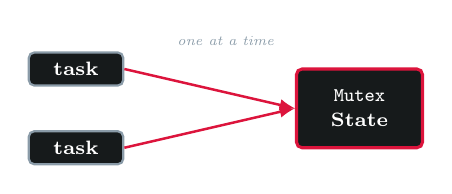
\begin{tikzpicture}[
        every node/.style={font=\scriptsize\bfseries},
        t/.style={
          draw=stplmuted, line width=0.8pt,
          fill=stplcard, text=stplwhite,
          rounded corners=2pt,
          minimum width=1.2cm, minimum height=0.42cm, align=center,
        },
        s/.style={
          draw=stplred, line width=1.1pt,
          fill=stplcard, text=stplwhite,
          rounded corners=2pt,
          minimum width=1.6cm, minimum height=1.0cm, align=center,
        },
        arr/.style={-latex, draw=stplred, line width=0.9pt},
        lbl/.style={font=\tiny\itshape, text=stplmuted},
      ]
      \node[t] (t1) at (0, 0.5)  {task};
      \node[t] (t2) at (0,-0.5)  {task};
      \node[s] (m)  at (3.6, 0)  {\texttt{Mutex}\\[1pt] State};
      \draw[arr] (t1.east) -- (m.west);
      \draw[arr] (t2.east) -- (m.west);
      \node[lbl] at (1.9, 0.85) {one at a time};
    \end{tikzpicture}
  \end{center}
  \vspace{-0.15cm}
  \begin{block}{The reflex}
\begin{lstlisting}
let vault = Arc::new(Mutex::new(0u64));
let v = Arc::clone(&vault);
tokio::spawn(async move { *v.lock().unwrap() += 100; });
\end{lstlisting}
  \end{block}
\end{frame}

\begin{frame}{The lock tax}
  \begin{itemize}
    \item The compiler checks that access is exclusive --- not that lock \textbf{order} is consistent
    \item Under contention, threads queue on one cache line and extra cores stop helping
  \end{itemize}
  \vspace{0.1cm}
  \begin{center}
    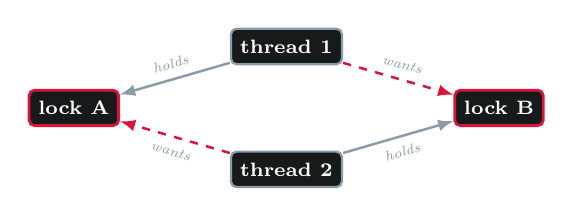
\begin{tikzpicture}[
        every node/.style={font=\scriptsize\bfseries},
        t/.style={
          draw=stplmuted, line width=0.8pt,
          fill=stplcard, text=stplwhite,
          rounded corners=2pt,
          minimum width=1.2cm, minimum height=0.45cm, align=center,
        },
        l/.style={
          draw=stplred, line width=1pt,
          fill=stplcard, text=stplwhite,
          rounded corners=2pt,
          minimum width=1.1cm, minimum height=0.45cm, align=center,
        },
        holds/.style={-latex, draw=stplmuted, line width=0.9pt},
        wants/.style={-latex, draw=stplred, line width=0.9pt, dashed},
        lbl/.style={font=\tiny\itshape, text=stplmuted},
      ]
      \node[l] (la) at (0,   0)     {lock A};
      \node[l] (lb) at (5.4, 0)     {lock B};
      \node[t] (t1) at (2.7, 0.78)  {thread 1};
      \node[t] (t2) at (2.7,-0.78)  {thread 2};

      \draw[holds] (t1) -- (la) node[midway, sloped, above, lbl] {holds};
      \draw[wants] (t1) -- (lb) node[midway, sloped, above, lbl] {wants};
      \draw[holds] (t2) -- (lb) node[midway, sloped, below, lbl] {holds};
      \draw[wants] (t2) -- (la) node[midway, sloped, below, lbl] {wants};
    \end{tikzpicture}
  \end{center}
  \begin{alertblock}{What ``safe'' actually covers}
    Safe Rust rules out data \textbf{races}. Deadlocks, race \textbf{conditions} and
    lock-order bugs remain fully safe, fully compiling, and fully yours.
  \end{alertblock}
\end{frame}

% <1-2>, not <1>: block/alertblock carry a \pause (preamble), so a single-overlay
% frame renders the helper block invisible. Overlay 1 = diagram, 2 = block.
\begin{frame}<1-2>{Mutex soup}
  \begin{center}
    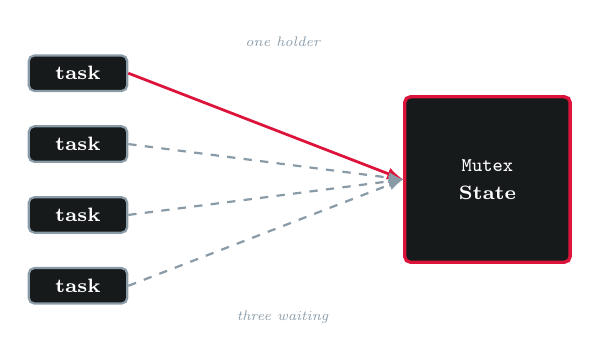
\begin{tikzpicture}[
        every node/.style={font=\scriptsize\bfseries},
        t/.style={
          draw=stplmuted, line width=0.8pt,
          fill=stplcard, text=stplwhite,
          rounded corners=2pt,
          minimum width=1.25cm, minimum height=0.45cm, align=center,
        },
        s/.style={
          draw=stplred, line width=1.2pt,
          fill=stplcard, text=stplwhite,
          rounded corners=2pt,
          minimum width=2.1cm, minimum height=2.1cm, align=center,
        },
        arr/.style={-latex, draw=stplred, line width=1pt},
        warr/.style={-latex, draw=stplmuted, line width=0.8pt, dashed},
        lbl/.style={font=\tiny\itshape, text=stplmuted},
      ]
      \node[t] (t1) at (0, 1.35) {task};
      \node[t] (t2) at (0, 0.45) {task};
      \node[t] (t3) at (0,-0.45) {task};
      \node[t] (t4) at (0,-1.35) {task};

      \node[s] (m) at (5.2, 0) {\texttt{Mutex}\\[2pt] State};

      \draw[arr]  (t1.east) -- (m.west);
      \draw[warr] (t2.east) -- (m.west);
      \draw[warr] (t3.east) -- (m.west);
      \draw[warr] (t4.east) -- (m.west);

      \node[lbl] at (2.6, 1.75) {one holder};
      \node[lbl] at (2.6,-1.75) {three waiting};
    \end{tikzpicture}
  \end{center}
  \vspace{0.1cm}
  \begin{exampleblock}{The smell}
    When \texttt{Arc<Mutex<T>>} shows up in five signatures, the state has no
    owner --- it has co-owners, and they negotiate at runtime.
  \end{exampleblock}
\end{frame}

% ================================================================
\section{The actor model}

\begin{frame}{What an actor is}
  \begin{itemize}
    \item An \textbf{actor} owns an address, a mailbox and private state --- nothing reaches inside
    \item The only way to affect it is to \textbf{send a message} to its address
    \item Sending is asynchronous --- the sender hands the message over and keeps running
    \item Handling one message, it may reply, spawn more actors, or change how it handles the next
  \end{itemize}
  \vspace{0.2cm}
  \begin{block}{The whole contract}
    One owner \textperiodcentered{} one mailbox \textperiodcentered{} one message at a time
  \end{block}
\end{frame}

\begin{frame}{The mailbox}
  \begin{center}
    \begin{tikzpicture}[
        every node/.style={font=\scriptsize\bfseries},
        t/.style={
          draw=stplmuted, line width=0.8pt,
          fill=stplcard, text=stplwhite,
          rounded corners=2pt,
          minimum width=1.1cm, minimum height=0.42cm, align=center,
        },
        slot/.style={
          draw=stplmuted, line width=0.7pt,
          fill=stplcard, text=stplwhite,
          minimum width=0.5cm, minimum height=0.5cm,
        },
        a/.style={
          draw=stplred, line width=1.2pt,
          fill=stplcard, text=stplwhite,
          rounded corners=2pt,
          minimum width=1.8cm, minimum height=1.5cm, align=center,
        },
        arr/.style={-latex, draw=stplred, line width=1pt},
        lbl/.style={font=\tiny\itshape, text=stplmuted},
      ]
      % Stage 1: the actor and its private state
      \node[a] (act) at (7.4, 0) {actor};
      \node[font=\tiny\bfseries, text=stplred] at (7.4,-0.42) {state};
      \node[lbl] at (7.4,-1.15) {private, unshared};

      % Stage 2: the mailbox
      \begin{scope}[visible on=<2->]
        \node[slot] (s1) at (3.9, 0) {};
        \node[slot] (s2) at (4.4, 0) {};
        \node[slot] (s3) at (4.9, 0) {};
        \node[lbl] at (4.4, 0.62) {mailbox};
      \end{scope}

      % Stage 3: senders push messages in
      \begin{scope}[visible on=<3->]
        \node[t] (p1) at (0.6, 0.85) {task};
        \node[t] (p2) at (0.6, 0)    {task};
        \node[t] (p3) at (0.6,-0.85) {task};
        \draw[arr] (p1.east) -- (s1.west);
        \draw[arr] (p2.east) -- (s1.west);
        \draw[arr] (p3.east) -- (s1.west);
        \node[lbl] at (2.4,-1.15) {send, never block on a lock};
      \end{scope}

      % Stage 4: the actor drains its mailbox, strictly in order
      \begin{scope}[visible on=<4->]
        \draw[arr] (s3.east) -- (act.west) node[midway, above, lbl] {one at a time};
      \end{scope}
    \end{tikzpicture}
  \end{center}
  \begin{itemize}
    \item<1-> State lives inside \textbf{one} actor and is never handed out
    \item<2-> Every message lands in a queue instead of contending for a lock
    \item<3-> Senders keep running --- delivery is asynchronous by construction
    \item<4-> The actor handles messages \textbf{sequentially}, so exclusion is free
  \end{itemize}
\end{frame}

% Choreographed (style.md 4.5b): every item pinned, revealing one at a time down
% the left column then the right. Pins start at <2->, not <1->: a boxed column
% emits nothing at all on overlay 1, so anything pinned there is lost. The <2-9>
% frame spec then trims that unusable leading page.
\begin{frame}<2-9>{Locks vs actors}
  % Raw tcolorbox rather than block/alertblock: those bake in a \pause, which
  % inside a boxed column costs a dead title-only overlay. Same branded styles,
  % reveal driven purely by the pinned \item overlays.
  \begin{columns}[T]
    \column{0.48\textwidth}
      \begin{tcolorbox}[stplbase, colframe=stplred!75!black,
        colback=stplred!10!stplcard, title={Locks}]
        \begin{itemize}
          \item<2-> State has co-owners
          \item<3-> Exclusion enforced at runtime
          \item<4-> Lock order is a global invariant
          \item<5-> A panic poisons the mutex
        \end{itemize}
      \end{tcolorbox}

    \column{0.48\textwidth}
      % \uncover, not bare: the card would otherwise sit empty from overlay 3.
      % \uncover keeps its geometry reserved, so nothing shifts when it lands.
      \uncover<6->{%
      \begin{tcolorbox}[stplbase, breakable=false, colframe=stplred, title={Actors}]
        \begin{itemize}
          \item<6-> State has exactly one owner
          \item<7-> Exclusion by construction
          \item<8-> Order is per-mailbox, local
          \item<9-> A panic kills one actor
        \end{itemize}
      \end{tcolorbox}}
  \end{columns}
  \vspace{0.15cm}
  \begin{center}
    \textcolor{stplmuted}{\small Same guarantee. One is checked by convention, the other by shape.}
  \end{center}
\end{frame}

% ================================================================
\section{What it buys}

\begin{frame}{Failure has a boundary}
  \begin{itemize}
    \item Shared state fails \textbf{globally} --- a poisoned mutex or a torn invariant reaches every caller
    \item An actor's blast radius is its own mailbox and its own state
    \item Recovery is a restart, not a repair, because there is nothing else to restore
    \item Testing narrows to: given this message sequence, what does one actor do
  \end{itemize}
  \vspace{0.2cm}
  \begin{exampleblock}{Effect}
    The unit of failure and the unit of reasoning become the \textbf{same} unit.
  \end{exampleblock}
\end{frame}

\begin{frame}[fragile]{Backpressure, free}
  \begin{itemize}
    \item A mailbox has a \textbf{capacity}, and a full mailbox suspends the sender
    \item Overload turns into waiting instead of unbounded memory growth
    \item The queue depth is a metric --- the system reports its own saturation
    \item Unbounded channels move the failure from the queue to the allocator
  \end{itemize}
  \begin{block}{Bounded on purpose}
\begin{lstlisting}
let (tx, rx) = mpsc::channel(32);  // 32 in flight, then wait

tx.send(msg).await?;               // suspends when full
\end{lstlisting}
  \end{block}
\end{frame}

\begin{frame}{Single-threaded reasoning}
  \begin{itemize}
    \item Inside the actor, exactly one message is in flight --- no interleaving to imagine
    \item Multi-step invariants hold, because nothing observes the middle of a step
    \item \texttt{\&mut self} is available for free, with no lock and no guard lifetime
    \item Concurrency moves to the \textbf{edges}: how actors are wired, not what they do
  \end{itemize}
  \vspace{0.2cm}
  \begin{block}{The trade}
    Sequential code inside, concurrency in the topology. Debugging a hard problem
    means reading \textbf{one} loop.
  \end{block}
\end{frame}

\begin{frame}{What a message costs}
  \begin{itemize}
    \item A lock is nanoseconds; a message adds an allocation and a wakeup
    \item Contention \textbf{grows} the lock's cost with cores --- actor state stays cache-hot
  \end{itemize}
  \vspace{-0.3cm}
  \begin{center}
    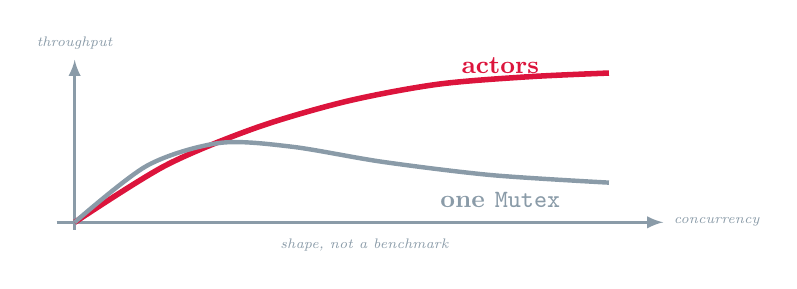
\begin{tikzpicture}[x=1.15cm, y=0.48cm,
        lbl/.style={font=\tiny\itshape, text=stplmuted}]
      \draw[draw=stplmuted, -latex, line width=1pt]
        (-0.2,0) -- (6.5,0) node[right, lbl] {concurrency};
      \draw[draw=stplmuted, -latex, line width=1pt]
        (0,-0.2) -- (0,4.3) node[above, lbl] {throughput};

      % actors: scales, then saturates
      \draw[draw=stplred, line width=2pt, smooth]
        plot coordinates {(0,0) (1,1.5) (2,2.5) (3,3.2) (4,3.65) (5,3.85) (5.9,3.95)};
      % one shared Mutex: peaks, then contention eats the gains
      \draw[draw=stplmuted, line width=1.6pt, smooth]
        plot coordinates {(0,0) (0.8,1.5) (1.6,2.1) (2.4,2.0) (3.4,1.6) (4.6,1.25) (5.9,1.05)};

      \node[font=\small\bfseries, text=stplred]   at (4.7, 4.15) {actors};
      \node[font=\small\bfseries, text=stplmuted] at (4.7, 0.6)  {one \texttt{Mutex}};
      \node[lbl] at (3.2,-0.6) {shape, not a benchmark};
    \end{tikzpicture}
  \end{center}
  \begin{block}{The trade}
    Worse latency per message, better throughput under contention.
  \end{block}
\end{frame}

\begin{frame}{When not to}
  \begin{itemize}
    \item A hot counter --- a message is an allocation and a queue hop, an atomic is nanoseconds
    \item Request/response cycles --- A asks B, B asks A, and deadlock is back across two files
    \item Global ordering --- guarantees are per sender/receiver pair, never system-wide
    \item Debugging --- stack traces stop at the channel and become log archaeology
  \end{itemize}
  \vspace{0.2cm}
  \begin{alertblock}{Honest framing}
    Actors are a \textbf{structuring} tool, not a performance tool. Reaching for
    one to speed up a counter trades nanoseconds for architecture.
  \end{alertblock}
\end{frame}

% ================================================================
\section{Actors in Rust}

\begin{frame}{Ownership is the fit}
  \begin{itemize}
    \item Rust's central rule --- one owner, or many readers, never both --- is the actor rule
    \item Sending a message \textbf{moves} it, so the sender provably cannot touch it again
    \item Holding a \texttt{std} guard across \texttt{.await} makes the future \texttt{!Send} and \texttt{spawn} rejects it
  \end{itemize}
  \vspace{-0.15cm}
  \begin{center}
    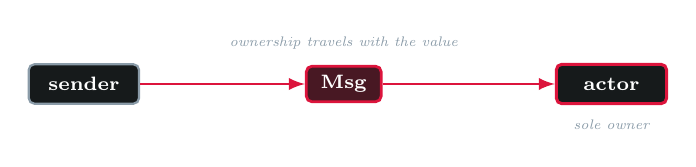
\begin{tikzpicture}[
        every node/.style={font=\scriptsize\bfseries},
        t/.style={
          draw=stplmuted, line width=0.8pt,
          fill=stplcard, text=stplwhite,
          rounded corners=2pt,
          minimum width=1.4cm, minimum height=0.5cm, align=center,
        },
        a/.style={
          draw=stplred, line width=1.1pt,
          fill=stplcard, text=stplwhite,
          rounded corners=2pt,
          minimum width=1.4cm, minimum height=0.5cm, align=center,
        },
        msg/.style={
          draw=stplred, line width=1pt,
          fill=stplred!25!stplcard, text=stplwhite,
          rounded corners=2pt,
          minimum width=0.95cm, minimum height=0.44cm,
        },
        arr/.style={-latex, draw=stplred, line width=1pt},
        lbl/.style={font=\tiny\itshape, text=stplmuted},
      ]
      \node[t]   (task) at (0,   0) {sender};
      \node[msg] (m)    at (3.3, 0) {Msg};
      \node[a]   (act)  at (6.7, 0) {actor};

      \draw[arr] (task.east) -- (m.west);
      \draw[arr] (m.east)    -- (act.west);

      \node[lbl] at (3.3, 0.52) {ownership travels with the value};
      \node[lbl] at (6.7,-0.52) {sole owner};
    \end{tikzpicture}
  \end{center}
  \begin{block}{The observation}
    Every fight with the borrow checker over shared mutable state is the language
    describing an actor boundary that is not there yet.
  \end{block}
\end{frame}

\begin{frame}[fragile]{The message is the API}
  \begin{itemize}
    \item No framework required --- an \texttt{enum}, a \texttt{loop} and a spawned task
    \item The message type \textbf{is} the actor's public interface, written down in one place
    \item A new capability is a new variant, and the compiler lists every site to update
  \end{itemize}
  \begin{block}{The protocol}
\begin{lstlisting}
enum Msg {
    Deposit(u64),
    Balance(oneshot::Sender<u64>),
}
\end{lstlisting}
  \end{block}
\end{frame}

\begin{frame}[fragile]{The loop is the actor}
  \begin{itemize}
    \item State is a plain local variable, owned by this task and nothing else
    \item \texttt{\&mut} is free here --- no lock, no guard, no lifetime to thread through
    \item \texttt{match} is exhaustive, so an unhandled message is a compile error
  \end{itemize}
  \vspace{-0.4cm}
  \begin{block}{vault.rs}
\begin{lstlisting}
async fn run(mut rx: mpsc::Receiver<Msg>) {
    let mut balance: u64 = 0;          // owned here, nowhere else
    while let Some(msg) = rx.recv().await {
        match msg {
            Msg::Deposit(n)  => balance += n,
            Msg::Balance(tx) => { let _ = tx.send(balance); }
        }
    }
}
\end{lstlisting}
  \end{block}
\end{frame}

\begin{frame}[fragile]{The handle}
  \begin{itemize}
    \item Callers never see \texttt{Msg} --- they get a cheap, \texttt{Clone}-able handle
    \item Cloning the handle shares the \textbf{address}, never the state
    \item \texttt{Msg} never leaks, so the protocol can change without touching callers
  \end{itemize}
  \vspace{-0.25cm}
  \begin{block}{A typed address}
\begin{lstlisting}
#[derive(Clone)]
pub struct Vault(mpsc::Sender<Msg>);

impl Vault {
    pub fn spawn() -> Self {
        let (tx, rx) = mpsc::channel(32);
        tokio::spawn(run(rx));
        Self(tx)
    }
}
\end{lstlisting}
  \end{block}
\end{frame}

\begin{frame}[fragile]{Asking for an answer}
  \begin{itemize}
    \item Fire-and-forget is the default; a reply needs a \textbf{return address}
    \item \texttt{oneshot} is exactly that --- a single-use channel shipped inside the message
    \item The \texttt{async} signature hides the protocol entirely from the caller
  \end{itemize}
  \begin{block}{Request/response}
\begin{lstlisting}
impl Vault {
    pub async fn balance(&self) -> u64 {
        let (tx, rx) = oneshot::channel();
        self.0.send(Msg::Balance(tx)).await.expect("actor gone");
        rx.await.expect("actor dropped the reply")
    }
}
\end{lstlisting}
  \end{block}
  \vspace{-0.15cm}
  \textcolor{stplmuted}{\tiny Pattern after Alice Ryhl, ``Actors with Tokio'', ryhl.io \textperiodcentered{} 2021}
\end{frame}

\begin{frame}{Send and Sync}
  \begin{itemize}
    \item \texttt{Send} --- the value may move to another thread; \texttt{Sync} --- a shared reference may
    \item \texttt{tokio::spawn} demands \texttt{Send + 'static}, so a message must be \textbf{self-contained}
    \item A message that smuggles in shared mutable state is a type error, not a review comment
    \item Both are auto-derived --- a type is \texttt{Send} exactly when its fields are, with nothing to forget
  \end{itemize}
  \vspace{0.2cm}
  \begin{exampleblock}{The punchline}
    Every other runtime \textbf{asks} its authors not to share state.
    Here the compiler refuses to build the program that does.
  \end{exampleblock}
\end{frame}

\begin{frame}{Frameworks}
  \begin{itemize}
    \item \texttt{actix} --- the veteran; the actor runtime \texttt{actix-web} grew out of
    \item \texttt{ractor} --- supervision trees, named registries, clustering
    \item \texttt{kameo} --- newer, async-first, ergonomic, with remote actors
    \item All three buy the same thing: lifecycle and supervision, not message passing
  \end{itemize}
  \vspace{0.2cm}
  \begin{block}{Default position}
    Most production actors in Rust are forty lines of \texttt{mpsc} and a
    \texttt{match}. A framework earns its dependency when supervision or a
    registry does.
  \end{block}
\end{frame}

% ================================================================
\begin{frame}{Summary}
  \begin{enumerate}
    \item \textbf{Locks} give exclusion at runtime, leaving order and contention to the author
    \item \textbf{Actors} give exclusion by shape --- one owner, one mailbox, one message
    \item \textbf{Isolation} pays out as failure boundaries, backpressure, sequential reasoning
    \item \textbf{Rust} enforces the model's core assumption in the type system, for free
    \item \textbf{Start} with a channel and a \texttt{match}; add a framework when supervision does
  \end{enumerate}
  \vspace{-0.1cm}
  \begin{exampleblock}{Takeaway}
    The actor model is not a library. It is the answer to the question the
    borrow checker keeps asking.
  \end{exampleblock}
\end{frame}

% ================================================================
\begin{frame}[plain]
  \begin{center}
    \vfill
    {\Huge\bfseries\color{stplwhite} gn}
    \vfill
  \end{center}
\end{frame}

\end{document}
